\documentclass[11pt, oneside]{article} 
\usepackage{geometry}
\geometry{letterpaper} 
\usepackage{graphicx}
	
\usepackage{amssymb}
\usepackage{amsmath}
\usepackage{parskip}
\usepackage{color}
\usepackage{hyperref}

\graphicspath{{/Users/telliott_admin/Tex/png/}}
% \begin{center} 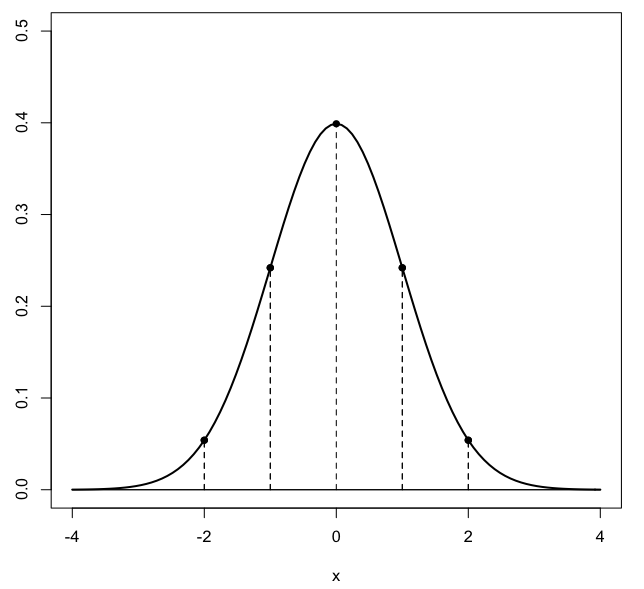
\includegraphics [scale=0.4] {gauss3.png} \end{center}

\title{Cardinality}
\date{}

\begin{document}
\maketitle
\Large

\section{Density}

We introduced the term \textbf{density} in discussion of the rational numbers and said that between any two rational numbers we can always find a third one, and gave a method for doing so.  The implication of this fact is that any particular interval like $[0,1]$ contains an infinite number of rationals.

We extend this now as follows:

\subsection*{theorem}

$\bullet$  Between any two \emph{real} numbers $a$ and $b$ it is always possible to find a rational number $r$:  
\[ \forall \ a,b \in \mathbb{R} \ \exists \ r \in \mathbb{Q} \ | \ r \in (a,b) \]

\subsection*{proof}

Pick $N \in \mathbb{N} \text{ such that }$
\[ N > b - a \]
\[ \frac{1}{N} < b - a \]

Let the set 
\[ \mathbf{A} = \{ \ \frac{m}{N}: \ m \in \mathbb{N} \} \]
so $\mathbf{A}$ is a subset of $\mathbb{Q}$.

Example:  suppose
\[ b = \pi = 3.14159265 \]
\[ a = e = 2.718281828 \]
the difference $b-a$ is less than $0.5$.  Pick $N = 10$ so
\[ \frac{1}{N} = 0.1 < 0.5 \]

The claim is that
\[ \mathbf{A} \cap (a,b) \ne \varnothing \]

There do exist numbers within the open interval $(a,b)$ that are in the set $\mathbf{A}$.

Assume on the contrary that the set $\mathbf{A}$ does not contain a rational number lying inside this interval.  In other words:

\[ \mathbf{A} \cap (e,\pi) = \varnothing \]

Now, find the largest integer $m_1$ such that 
\[ \frac{m_1}{N} < a \]
(it is OK if $m_1$ is equal to $0$).  For this example, that would be $27$, since $27/10 = 2.7 < e < 2.8$.

Then the next rational number in $\mathbf{A}$ must be larger than $b$ if the set intersection is empty.  For this example, we are claiming that $2.8$ does not lie in the interval $(e, \pi)$.

Formally, we claim that
\[ \frac{m_1 + 1}{N} > b \]

But this implies that
\[ \frac{m_1 + 1}{N} - \frac{m_1}{N} > b - a \]
\[ \frac{1}{N} > b - a \]
which contradicts our condition on $N$ above.  Hence the assumption is false and so
\[ \mathbf{A} \cap (a,b) \ne \varnothing \]
Thus there must exist a rational number $r$ in $\mathbf{A}$ such that $a < r < b$.

And clearly, it is false that $2.8$ does not lie in the interval $(e, \pi)$.

\subsection*{example}

Consider the open interval:  $(\sqrt{2},\sqrt{3})$.  
\[ a = \sqrt{2} \approx 1.414 \]
\[ b = \sqrt{3} \approx 1.732 \]
\[ b-a \approx 0.3178 \]
\[ \frac{1}{b-a} \approx 3.1462 \]
Pick $N \ge 4$, for example
\[ N = 4: \ \ \  1.414 < \frac{6}{4} = 1.5 < 1.732 \]
\[ N = 5: \ \ \  1.414 < \frac{8}{5} = 1.6 < 1.732 \]
\[ N = 6: \ \ \  1.414 < \frac{9}{6} = 1.5 < 1.732 \]
(In this case $N=2$ and $N=3$ happen to work as well).

\subsection*{ordering}
The real numbers can also be ordered.  A simple way is to use the rational numbers as a scaffold or guide.  Since we can always find a rational number $r$ that lies in the interval between any two real numbers $a$ and $b$ such that 
\[ r \in (a,b) \]

Then either $a < r < b$ or $b < r < a$ and so
\[ r < b \ \iff \ a < b \]
which orders $a$ and $b$.

\subsection*{density again}
We showed previously that we can always find a rational number that lies in the interval between either two rational numbers or two real numbers.  Now we prove the same assertion for real numbers in an interval.

\subsection*{theorem}

$\bullet$  Between any two rational numbers it is always possible to find a real number.  Courant says it "is not so obvious,;  we shall accept it as a basic axiom."

\[ \forall \ a,b \in \mathbb{Q} \ \exists \ c \in \mathbb{R} \ | \ c \in (a,b) \]

One proof consists of finding a \emph{particular} irrational in the interval $(a,b)$, where $a$ and $b$ are arbitrary rational numbers.  For $a < b$, we simply add to the number $a$ the following
\[ c = \frac{\sqrt{2}}{2}(b - a) \]

$c$ is smaller than $b - a$ (because $\sqrt{2}/2 < 1$) so the result $a + c$ lies between $a$ and $b$.  

We also know that $c$ is irrational, because $\sqrt{2}$ times any rational number is irrational.  Finally, $a + c$ is irrational because adding $\sqrt{2}$ times a rational number to any rational number produces an irrational number.

\subsection*{preliminary lemmas}  

$\sqrt{2}$ times a rational is irrational.  Suppose for integer $p, q, r, s$ we have
\[ \sqrt{2} \frac{p}{q} = \frac{r}{s} \]
then
\[ \sqrt{2} = \frac{rq}{ps} \]
But the right-hand side is rational, so this is a contradiction.

For the second requirement, again by contradiction suppose
\[ \sqrt{2} \ \frac{p}{q} +  \frac{s}{t} = \frac{u}{v} \]
for integer $p, q, r, s, u, v$.  But the right-hand side of
\[ \sqrt{2} = \frac{q}{p} ( \frac{u}{v} - \frac{s}{t}) \]
is rational, so this is a contradiction.

Note that powers are different.  What do you think about
\[ r = \sqrt{2}^{\sqrt{2}} \]
You may think $r$ is "likely" to be irrational.  Just a mess.  But how about
\[ r^{\sqrt{2}} \]
Whether $r$ is rational or irrational
\[ r^{\sqrt{2}} = (\sqrt{2}^{\sqrt{2}})^{\sqrt{2}} = \sqrt{2}^2 = 2 \]

\subsection*{theorem}

$\bullet$  Finally, between any two real numbers it is always possible to find another real number.  
\[ \forall \ a,b \in \mathbb{R} \ \exists \ c \in \mathbb{R} \ | \ c \in (a,b) \]

This one is subtle.  Suppose the two real numbers are "really, really close."  

\subsection*{proof}

We suppose that they are not equal, so they must be different, say $a < b$.

Since they are different, at some stage in the decimal expansions of $a$ and $b$, there must be a first position at which $a$ and $b$ differ.  If $b$ does not have a $0$ at the next position, terminate there and that will be $c$.

For example:
\[ a = 1.23456789129.. \]
\[ b = 1.23456789133.. \]
\[ c = 1.23456789130.. \]

$b$ must have some digit following this first position where it does not match $a$, and which is also not equal to zero (otherwise it would be a terminating decimal and thus a rational number).  So we can always find a place to terminate to form $c$.

Just to be clear, suppose we are interested in the \emph{smallest} number that is larger than $0$.  Well
\[ 1 > 0 \]
But, by this result, we can always find a number $a$ smaller than any given $b > 0$ such that $0 < a < b$.  There is no last number before $0$ when going to the left (or to the right) of the number.  Neither is there any last number just smaller than $\pi$ or $e$.

\subsection*{nested intervals}
Courant and John set up a system in which real numbers are specified as a nested sequence of intervals with rational bounds.
\begin{center} 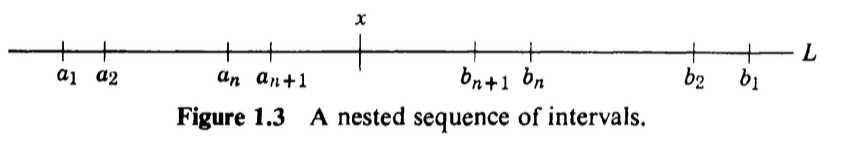
\includegraphics [scale=0.5] {nested_intervals.png} \end{center}
with 
\[ a_1 \le a_2 \le a_3 \le x \le b_3 \le b_2 \le b_1 \]

They say
\begin{quote}let $x$ be confined to a closed interval $I_1 = [a_1,b_1]$ where $a_1$ and $b_1$ are rational.  Within $I_1$ we consider a "subinterval" $I_2 = [a_2,b_2]$ containing $x$, where $a_2$ and $b_2$ are rational.  For example, we may choose for $I_2$ one of the halves of $I_1$, for $x$ must lie in one or both of the halves of $I_1$.  Within $I_2$ we consider a subinterval $I_3 = [a_3,b_3]$ ...  We require that the length of the interval $I_n$ tends to zero with increasing $n$;  that is that the length of $I_n$ is less than any preassigned positive number for all large $n$ ...  A set of closed intervals $I_1, I_2, I_3 \dots$ each containing the next one and such that the lengths tend to zero will be called a "nested sequence of intervals."  The point $x$ is uniquely determined by the nested sequence ... we see that every point $x$, that is, every real number, can be precisely described with the help of infinitely many rational numbers.\end{quote}

\begin{center} 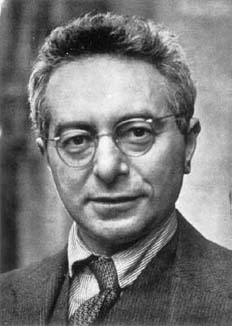
\includegraphics [scale=0.5] {Courant_3.png} \end{center}
Courant

The quote above continues:
\begin{quote}As we shall see, this is an \emph{axiom of continuity}:  it guarantees that no gaps exist on the real axis.  We shall use the axiom to characterize the real continuum and to justify all operations with limits which are basic for calculus and analysis.  (There are also many other ways of formulating this axiom ...)\end{quote}

Compare this description with the process of approximating $\sqrt{2}$ by writing its decimal expansion.

\section{Cantor and countability}

\textbf{Eternity is a very long time, especially towards the end. }

(credited to Woody Allen)

\subsection*{infinity}

The supply of natural numbers $\mathbb{N}$ is infinite, because if not, then there would be a maximum integer $m \in \mathbb{N}$.  But $m + 1$ is also $\in \mathbb{N}$, and $m+1 > m$, which is a contradiction.

Both the real numbers and the rational numbers also come in an infinite supply, for basically the same reason.  Just add $1$ to the "maximum" $m$, then find a real or a rational in the interval $(m,m+1)$.  

Even for a finite interval such as $(0,1)$, the properties described above prove that this finite interval contains an infinite number of both rational and real numbers.

But more than this, in an important sense, there are \emph{many more} real numbers than rational numbers.

\subsection*{more reals}

\url{www-history.mcs.st-and.ac.uk/~john/analysis/Lectures/L4.html}

The set $\mathbb{N}$ is \textbf{countable}.  Any set that can be put into one-to-one correspondence with $\mathbb{N}$ is also countable.

The set $\mathbb{Z}$ is countable:

\begin{center} 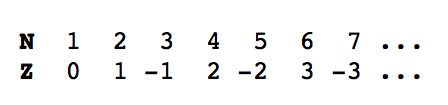
\includegraphics [scale=0.5] {Z_count.png} \end{center}

The set $\mathbb{N \times N}$ is countable:

\begin{center} 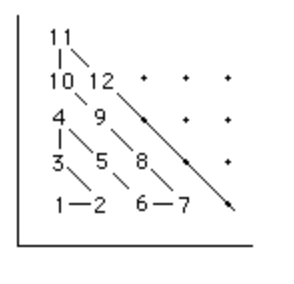
\includegraphics [scale=0.5] {countable.png} \end{center}

Count the points with integer coefficients in the positive quadrant as shown above.

The set $\mathbb{Q}$ is countable:

The idea of the proof is to show that one can set up a correspondence between $\mathbb{N}$ and $\mathbb{Q}$, assigning each number $r \in \mathbb{Q}$ in a particular order to $1,2,3, \dots$.  Here is the figure from Courant and John:
\begin{center} 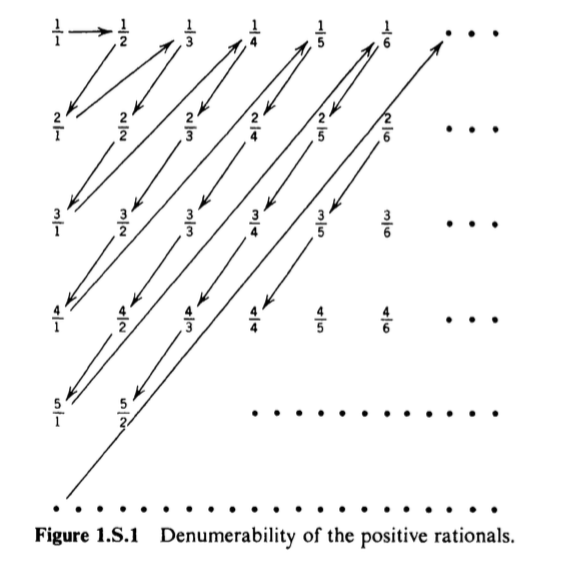
\includegraphics [scale=0.6] {denumerability.png} \end{center}

We first set up the sequence
\[ \frac{1}{1} \ \ \ \frac{1}{2}, \frac{2}{1} \ \ \  \frac{1}{3}, \frac{2}{2}, \frac{3}{1} \ \ \ \frac{1}{4}, \frac{2}{3}, \frac{3}{2}, \frac{4}{1} \ \ \ \frac{1}{5}, \frac{2}{4}, \frac{3}{3}, \frac{4}{2}, \frac{5}{1} \ \ \  \frac{1}{6}, \frac{2}{5}, \frac{3}{4}, \frac{4}{3}, \frac{5}{2}, \frac{6}{1} \dots \]
Then we remove all fractions that are duplicates by way of not being in lowest terms.
\[ \frac{1}{1} \ \ \ \frac{1}{2}, \frac{2}{1} \ \ \  \frac{1}{3}, \frac{3}{1} \ \ \ \frac{1}{4}, \frac{2}{3}, \frac{3}{2}, \frac{4}{1} \ \ \ \frac{1}{5}, \frac{5}{1} \ \ \  \frac{1}{6}, \frac{2}{5}, \frac{3}{4}, \frac{4}{3}, \frac{5}{2}, \frac{6}{1} \dots \]

Finally, each $r$ in this sequence is assigned to a natural number (in the sequence $\mathbb{N}$), establishing the denumerability property.

Cantor showed that such a correspondence is impossible for $\mathbb{R}$.  The proof of this is is not hard.  You can check out the chapters on Georg Cantor in Dunham's \emph{Journey Through Genius}.

We will show that the set of reals in the interval $(0,1)$ is not countable.

The proof is called the \emph{Cantor diagonalization argument}.

Suppose we could write down all the decimal expansions of the reals in the interval $(0,1)$ in a list:

- $0. a_1 \ a_2 \ a_3 \ a_4 \ a_5 \dots$

- $0. b_1 \ b_2 \ b_3 \ b_4 \ b_5 \dots$

- $0. c_1 \ c_2 \ c_3 \ c_4 \ c_5 \dots$

- $0. d_1 \ d_2 \ d_3 \ d_4 \ d_5 \dots$

$\dots$

Then this list would be countable, but it does not contain all the reals in the interval $(0,1)$

Define a decimal $x = x_1 \ x_2 \ x_3 \ x_4 \ \dots$, with $x_1 \ne a_1$ and also $x_1 \ne 9$ (so $x$ doesn't end in recurring $9$'s), then $x_2 \ne b_2,9$, $x_3 \ne c_3,9$, etc.

Then the decimal expansion of $x$ does not end in recurring $9$'s and it differs from the nth element of the list in the nth decimal place. Hence it represents an element of the interval (0, 1) which is not in our counting.

This means that we do not have a counting of the reals in (0, 1).

The rational numbers are said to be "countably infinite", while the real numbers are infinite but not countable.  In this sense there are more real numbers than rational numbers, and more irrational than rational numbers.

\subsection*{transcendental numbers}

A real number is called algebraic if it is a root of a polynomial with rational (or integer) coefficients. Real numbers that cannot be so expressed are called transcendental.  Both $\pi$ and $e$ are transcendental.

One final surprise:  Cantor showed that the algebraic numbers \emph{are} countable. Since the real numbers are not, the transcendental numbers are also non-countable, and thus much more numerous than the algebraic ones.

\subsection*{cardinality}

Countability or correspondence is described more formally as cardinality.  For the definition we consider two sets and a function $f : \mathbf{A} \rightarrow \mathbf{B}$.

Recall that a function is onto or \emph{surjective} if every element of $\mathbf{B}$ appears in the image of $f$, that is, for every $b \in \mathbf{B}$ there is some $a \in \mathbf{A}$ such that $f(a) = b$.  The image and the codomain of the function are the same.

And a function is one-to-one or \emph{injective} if $f(x) = b$ and $f(y) = b$ implies that $x = y$.  For every $b$ in the image of $f$ there is a unique $a$ such that $f(a) = b$.

A function is bijective if it has both properties:  every element of $\mathbf{A}$ is mapped by $f$ to a unique element of $b \in \mathbf{B}$, and for every element of $\mathbf{B}$ there is an $a$ such that $f(a) = b$.

We say that two non-empty sets $\mathbf{A}$ and $\mathbf{B}$ have the same cardinality if there is a function that is both one-to-one and onto.  In this case we write $\mathbf{A}$ [tilde symbol] $\mathbf{B}$.

\subsection*{example}

A somewhat shocking example is that $(0,1)$ and $(0,\infty)$ have the same cardinality.  We demonstrate this by finding a function that assigns to every number in $(0,1)$ a number in $(0,\infty)$.

\begin{center} 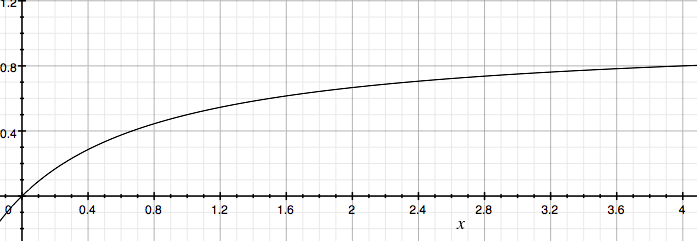
\includegraphics [scale=0.4] {mapping.png} \end{center}

That function is 
\[ y = \frac{x}{x+1} \]

\end{document}